\documentclass[../Main.tex]{subfiles}

\begin{document}
\subsection{Processing and Cleaning the Data}
In order to make predictions the authors decided that the PdDistrict would suffice as location information, so the address could be dropped. The description and resolution of the crime and arrest were also unnecessary to make a description of the type of crime.
The authors changed the date into numbers and splitted into separate columns consisting of Year, month, day, hour and DayOfWeek.

While plotting the cooridinates, some outliers were noticeable.

\begin{figure}[H]
\centering
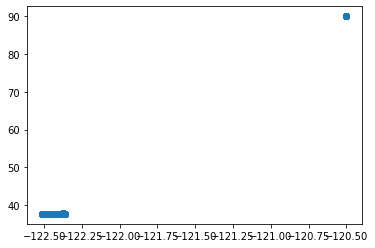
\includegraphics[width=0.3\textwidth]{Resources/PlotCooridinates.png}
\caption{\label{fig:PlotCooridinates}Plot of Cooridinates.}
\end{figure}

Since San Francisco has the latitude of circa 37, all coordinates with latitude under 40 were kept and the rest deleted, there were only 76 coordinates to be deleted. 

\begin{figure}[H]
\centering
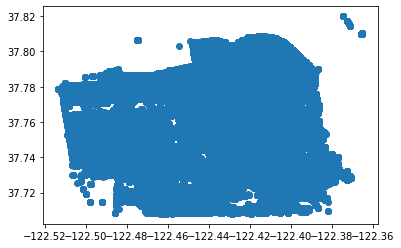
\includegraphics[width=0.3\textwidth]{Resources/CleanedCoordinates.png}
\caption{\label{fig:CleanedCoordinates}Plot of Cooridinates cleaned up.}
\end{figure}

\subsubsection{Binning}
To make the patterns more noticeable the authors decided to use Data binning. 
The Hours were binned in an equal-width size 6 bin, the divisions represent Early morning, morning, noon, afternoon, evening and night.
Additionaly the longitude and latitude were binned separately in size 80 bins.
\end{document}